\documentclass[tikz,border=2pt]{standalone}
\usepackage{amsmath}
\usetikzlibrary{arrows.meta}
\begin{document}
% Two ways out of a function body: an early return() for bad input leaves at once (code after it
% is never run); otherwise the body runs to its last expression, whose value is returned.
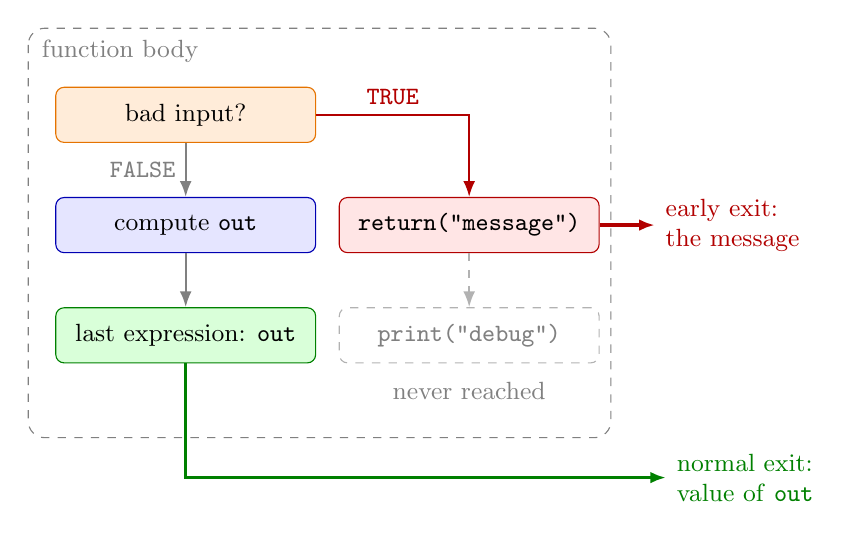
\begin{tikzpicture}[font=\small, >={Latex[length=2mm]},
  box/.style={draw, rounded corners=3pt, align=center, inner sep=4pt, minimum height=7mm, minimum width=3.3cm}]
  \draw[gray, dashed, rounded corners=6pt] (-2.0,0.75) rectangle (5.4,-4.45);
  \node[gray, anchor=north west] at (-1.95,0.72) {function body};
  \node[box, draw=orange!90!black, fill=orange!15] (t) at (0,-0.35) {bad input?};
  \node[box, draw=blue!70!black, fill=blue!10] (c) at (0,-1.75) {compute \texttt{out}};
  \node[box, draw=green!50!black, fill=green!15] (l) at (0,-3.15) {last expression: \texttt{out}};
  \node[box, draw=red!70!black, fill=red!10] (r) at (3.6,-1.75) {\texttt{return("message")}};
  \node[box, draw=gray!60, dashed, text=gray] (p) at (3.6,-3.15) {\texttt{print("debug")}};
  \node[gray, font=\small] at (3.6,-3.85) {never reached};
  \draw[->, thick, gray] (t) -- node[left, font=\small\ttfamily] {FALSE} (c);
  \draw[->, thick, gray] (c) -- (l);
  \draw[->, thick, red!70!black] (t.east) -| node[pos=0.25, above, font=\small\ttfamily] {TRUE} (r.north);
  \draw[->, thick, gray!60, dashed] (r) -- (p);
  % exits to the caller
  \draw[->, very thick, red!70!black] (r.east) -- ++(0.7,0) node[right, align=left] {early exit:\\ the message};
  \draw[->, very thick, green!50!black] (l.south) -- ++(0,-1.45) -- ++(6.1,0) node[right, align=left] {normal exit:\\ value of \texttt{out}};
\end{tikzpicture}
\end{document}
